\chapter{Analyse des Besoins et Conception}

\section{Collecte des exigences}
La phase d'analyse a débuté par une série d'entretiens avec cinq PME de différents secteurs d'activité. Ces entretiens ont permis d'identifier les fonctionnalités prioritaires. Comme le souligne \cite{martin2017clean}, une analyse rigoureuse des besoins est essentielle pour concevoir une architecture adaptée.

\begin{table}[H]
	\centering
	\caption{Priorisation des fonctionnalités demandées}
	\begin{tabular}{p{8cm}c}
		\toprule
		\textbf{Fonctionnalité} & \textbf{Priorité}\\
		\midrule
		Gestion des tâches et sous-tâches & Élevée \\
		Tableaux Kanban & Élevée \\
		Gestion du temps et suivi & Moyenne \\
		Rapports et statistiques & Moyenne \\
		Intégration calendrier & Faible \\
		\bottomrule
	\end{tabular}
\end{table}

\section{Architecture technique}
L'architecture retenue suit le pattern MVC (Model-View-Controller) avec une séparation claire entre le frontend et le backend. Cette approche s'inspire des principes d'architecture propre défendus par \cite{martin2017clean}.

\begin{figure}[H]
	\centering
	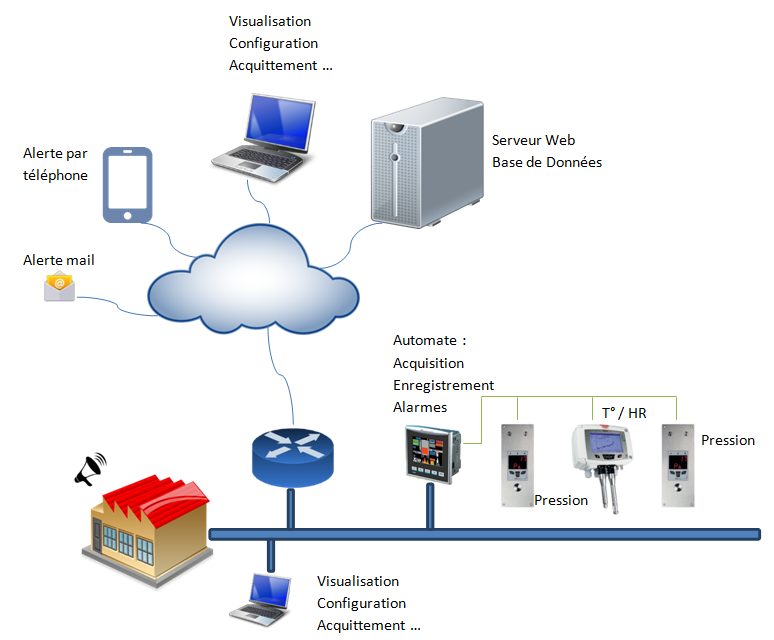
\includegraphics[width=0.8\textwidth]{images/architecture.png}
	\caption{Architecture globale du système}
	\label{fig:architecture}
\end{figure}

\subsection{Frontend}
Le frontend utilise React avec TypeScript pour une meilleure maintenabilité du code. Les principales librairies utilisées sont :
\begin{itemize}
	\item React 18 avec hooks \cite{react2024}
	\item TypeScript pour le typage statique
	\item Material-UI pour les composants d'interface
	\item React Query pour la gestion des états serveur
\end{itemize}

Le choix de React \cite{react2024} s'est imposé pour sa large adoption et sa riche ecosysteme de composants.

\subsection{Backend}
Le backend est développé en Node.js avec Express.js et utilise une base de données PostgreSQL. Node.js \cite{nodejs2024} a été choisi pour sa performance et sa compatibilité avec JavaScript côté serveur.

\begin{table}[H]
	\centering
	\caption{Stack technique complète}
	\begin{tabular}{p{6cm}p{8cm}}
		\toprule
		\textbf{Composant} & \textbf{Technologie} \\
		\midrule 
		Frontend & React 18, TypeScript, Material-UI, Vite \\
		Backend & Node.js \cite{nodejs2024}, Express.js, TypeScript \\ 
		Base de données & PostgreSQL avec Prisma ORM \\
		Authentification & JWT avec refresh tokens \\
		Déploiement & Docker, AWS ECS \\
		\bottomrule
	\end{tabular}
\end{table}

L'architecture globale respecte les principes REST définis par \cite{fielding2000rest}, garantissant une API stateless et scalable.